% =====================================================================
%  A1 PORTRAIT POSTER (594 x 841 mm)
%  Energy-Aware Arm and Base Selection for a Dual-Gantry Quad-Arm
%  Ceiling Robot Using a GNG Map
%
%  All content/numbers come from energy_aware_selection.tex (6-page paper).
%  Layout mimics the TMU Term-End Evaluation poster template:
%  orange rounded frame + rounded section pills + two columns.
%
%  Build:  pdflatex poster_energy_aware_A1.tex
%
%  Tuning knobs (top of preamble): \bodysize / \bodyskip control all body
%  text; \IG{<frac>}{<file>} scales every figure by \figscale.
% =====================================================================
\documentclass[20pt,a4paper]{extarticle}

\usepackage[
  paperwidth=594mm, paperheight=841mm,
  left=14mm, right=14mm, top=13mm, bottom=13mm
]{geometry}

\usepackage[T1]{fontenc}
\usepackage[utf8]{inputenc}
\usepackage[scaled=0.98]{helvet}
\renewcommand{\familydefault}{\sfdefault}

\usepackage{amsmath,amssymb}
\usepackage{graphicx}
\usepackage{xcolor}
\usepackage[most]{tcolorbox}
\usepackage{tikz}
\usetikzlibrary{positioning,calc,arrows.meta}
\usepackage{eso-pic}
\usepackage{enumitem}
\usepackage{booktabs}
\usepackage{array}
\usepackage{ragged2e}
\usepackage{anyfontsize}

\graphicspath{{figure/}}

% ------------------------------------------------------------- knobs
\newcommand{\bodysize}{17}
\newcommand{\bodyskip}{21}
\newcommand{\pillsize}{25}
\def\figscale{0.95}                       % global figure scale
\newcommand{\IG}[2]{\includegraphics[width=\figscale\dimexpr#1\linewidth\relax]{#2}}

% ---------------------------------------------------------------- colors
\definecolor{pgold}{HTML}{F5B335}   % section pill / frame
\definecolor{pgoldd}{HTML}{D98C0F}  % darker gold
\definecolor{pbody}{HTML}{1A1A1A}
\definecolor{pblue}{HTML}{1F4E79}   % accent for key numbers
\definecolor{pgrey}{HTML}{6E6E6E}

\color{pbody}
\setlength{\parindent}{0pt}
\setlength{\parskip}{3pt}
\renewcommand{\arraystretch}{1.12}

% ------------------------------------------------- outer rounded frame
\AddToShipoutPictureBG{%
  \begin{tikzpicture}[remember picture, overlay]
    \draw[pgold, line width=3.2pt, rounded corners=16pt]
      ($(current page.south west)+(8mm,8mm)$)
      rectangle
      ($(current page.north east)+(-8mm,-8mm)$);
  \end{tikzpicture}%
}

% ------------------------------------------------------ section pill
\newtcolorbox{sectionpill}{
  enhanced, width=\linewidth,
  colback=pgold, colframe=pgold,
  arc=8mm, boxrule=0pt,
  left=4mm, right=4mm, top=1.2mm, bottom=1.2mm,
  halign=flush center, valign=center,
  before skip=5mm, after skip=2.5mm
}
\newcommand{\psection}[1]{%
  \begin{sectionpill}\bfseries\fontsize{\pillsize}{\pillsize}\selectfont #1\end{sectionpill}}

% ------------------------------------------------------ highlight box
\newtcolorbox{keybox}{
  enhanced, width=\linewidth,
  colback=pgold!16!white, colframe=pgold,
  arc=4mm, boxrule=1.4pt,
  left=4mm, right=4mm, top=2.5mm, bottom=2.5mm,
  before skip=3mm, after skip=3mm
}

% ------------------------------------------------------ list styles
\setlist[itemize,1]{leftmargin=6.5mm, topsep=1pt, itemsep=2pt,
                    parsep=0pt, label=\textcolor{pgoldd}{$\bullet$}}
\setlist[itemize,2]{leftmargin=6mm, topsep=1pt, itemsep=1pt,
                    parsep=0pt, label=\textcolor{pgoldd}{$\circ$}}

% ------------------------------------------------------ helpers
\newcommand{\figcap}[1]{{\par\vspace{0.8mm}\centering
  \fontsize{14}{17}\selectfont\itshape\color{pgrey}#1\par\vspace{0.8mm}}}
\newcommand{\num}[1]{\textcolor{pblue}{\bfseries #1}}
\newcommand{\lead}[1]{\textbf{#1}}

\pagestyle{empty}

\begin{document}
\fontsize{\bodysize}{\bodyskip}\selectfont

% =====================================================================
%  HEADER
% =====================================================================
\begin{tcolorbox}[enhanced, width=\linewidth,
  colback=white, colframe=pgold, arc=10mm, boxrule=2.6pt,
  left=6mm, right=6mm, top=2mm, bottom=2mm]
\begin{minipage}[c]{0.085\linewidth}
  \centering
  \bfseries\fontsize{34}{34}\selectfont P-XX
\end{minipage}%
\begin{minipage}[c]{0.79\linewidth}
  \centering
  {\bfseries\fontsize{18}{21}\selectfont
   2026 The Term-End Evaluation, Department of Mechanical Systems Engineering, TMU.\par}
  \vspace{2mm}
  {\bfseries\fontsize{36}{42}\selectfont
   Energy-Aware Arm and Base Selection for a\\
   Dual-Gantry Quad-Arm Ceiling Robot\\
   Using a GNG Capability Map\par}
  \vspace{2.5mm}
  {\bfseries\fontsize{22}{26}\selectfont
   Naoyuki Kubota Laboratory, D2, Raditya Artha Rochmanto\par}
  {\fontsize{18}{22}\selectfont
   email: rochmanto-artha@ed.tmu.ac.jp\par}
\end{minipage}%
\begin{minipage}[c]{0.125\linewidth}
  \centering
  
\includegraphics[width=1\linewidth]{tmu_logo.jpg}\\[1.5mm]
  {\bfseries\fontsize{14}{16}\selectfont\color{pgrey} CONFIDENTIAL}
\end{minipage}
\end{tcolorbox}

% ------------------------------------------------------------- tagline
\begin{center}
  \bfseries\fontsize{23}{27}\selectfont
  Which arm should act, and where should its base go?\\
  One energy cost $J$, one base-aware capability map, both answers at once.
\end{center}

\vspace{-1mm}

% =====================================================================
%  TWO COLUMNS
% =====================================================================
\noindent
\begin{minipage}[t]{0.487\linewidth}
% ================================================= LEFT COLUMN =======

\psection{Social Background}

\begin{minipage}[t]{0.33\linewidth}
  \vspace{0pt}
  \IG{1.0}{ceilingarm_tll-edit.jpg}
\end{minipage}\hfill
\begin{minipage}[t]{0.64\linewidth}
  \vspace{0pt}\RaggedRight
  An aging population is driving demand for assistive robots that work
  \textbf{inside the home}: fetching, tidying, delivering.

  \vspace{2mm}
  Homes are small, cluttered, and \textbf{shared with residents}, so a
  floor-driving mobile manipulator gets in the way.

  \vspace{2mm}
  \textbf{Putting the robot on the ceiling} keeps the floor free: it assists
  from above without blocking the occupant.

  \vspace{2mm}
  \lead{Platform.} Two ceiling rails (gantries), \textbf{two Kinova Gen3 Lite
  arms each} $\rightarrow$ four arms.
\end{minipage}

\vspace{1.5mm}
Each rail adds a prismatic axis $d$ and a revolute axis $\theta$ that its two
arms \emph{share}, so every arm is an \textbf{8-DOF} chain
$\mathbf{q}=[d,\theta,q_1\ldots q_6]$ and moving the base moves two arms at once.

\psection{Problems}

\begin{itemize}
  \item \lead{P1 --- Two coupled decisions.} Each pick asks \emph{which arm}
        acts \emph{and where its base stops}. Moving the heavy base is a
        dominant energy cost.
  \item \lead{P2 --- Maps assume a fixed base.} Classic reachability/capability
        maps are built for one arm on a stationary base, so they never see the
        workspace that base motion creates.
  \item \lead{P3 --- A cell is only one bit.} Maps store \emph{whether} a cell
        is reachable, not at what cost or from which configuration: no IK seed,
        no arm choice.
\end{itemize}

\psection{Core Concept: Base-Aware GNG Capability Map}

\begin{itemize}
  \item Sample the \textbf{full 8-DOF} $\mathbf{q}=[d,\theta,q_1\ldots q_6]$
        inside joint limits, take forward kinematics (Pinocchio), record
        manipulability $w=\sqrt{\det(JJ^{\!\top})}$.
  \item Fit a \textbf{Growing Neural Gas} net: each node stores
        $[\,\mathbf{x}\mid\mathbf{q}\,]$ --- a reachable point \emph{and} a
        representative configuration reaching it, \textbf{rail placement
        included}.
  \item Winner search uses the \emph{task} part only (nodes tile the workspace);
        adaptation updates the whole vector, so a node's $\mathbf{q}$ stays one
        valid posture, not an average of incompatible base positions.
  \item \textbf{Boundary seeding}: a shell of nodes is pinned on the measured
        reach surface \emph{before} the interior grows, keeping the map faithful
        at the workspace edge.
  \item One map per arm $\rightarrow$ four maps, queried independently at
        selection time.
\end{itemize}

\vspace{1mm}
{\centering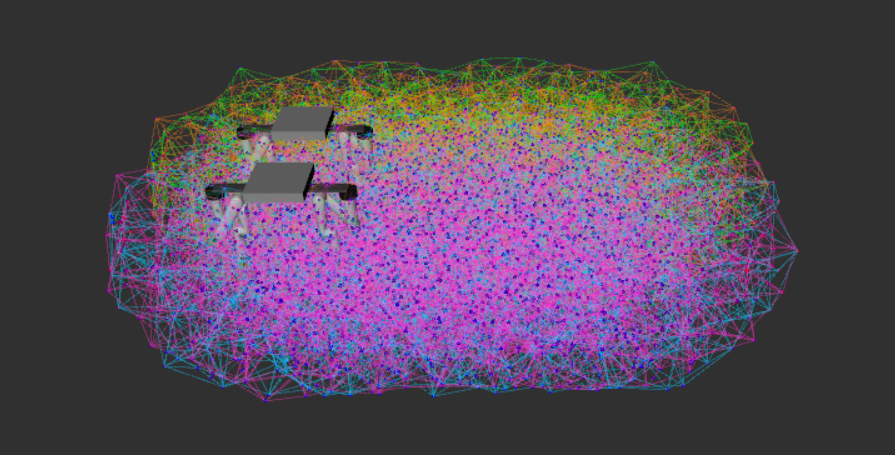
\includegraphics[trim=95 45 90 45, clip,
   width=\figscale\dimexpr0.62\linewidth\relax]{gng_capability.png}\par}
\figcap{Base-aware GNG map of one arm (RViz): nodes coloured by manipulability
plus the pinned boundary shell on the true rail-extended reach surface. The
elongated extent is the rail sweeping $x$.}

\begin{keybox}
\lead{E0 --- map built per arm:} 80{,}000 FK samples $\rightarrow$
\num{2915 nodes} (600 pinned on the boundary shell), 14{,}547 edges, median node
spacing \num{0.090~m}, and a full \num{8-DOF} $\mathbf{q}$ stored on every node.
\end{keybox}

\psection{Energy-Aware Selection Cost $J$}

\begin{keybox}
\centering
$\displaystyle
J = w_{gl}\frac{\Delta_{lin}}{\rho_{gl}}
  + w_{gr}\frac{\Delta_{rot}}{\rho_{gr}}
  + w_{arm}\frac{\Delta_{arm}}{\rho_{arm}}
  + w_{dist}\frac{e}{\rho_{dist}}
  - w_{manip}\frac{m}{\rho_{manip}}$
\end{keybox}

\begin{itemize}
  \item $\Delta_{lin},\Delta_{rot},\Delta_{arm}$: rail-linear, rail-rotation and
        summed arm-joint travel from the current state; $e$: tool-to-object
        distance; $m$: manipulability, entering \emph{negatively} --- dexterous
        is cheap.
  \item Each term is divided by a reference $\rho$ (its median over a
        calibration set), so a weight reads as a priority, not a unit artefact.
  \item Weights are \textbf{fit by OLS} against the \emph{measured} mechanical
        energy of 168 executed picks, not hand-tuned.
\end{itemize}

\vspace{1mm}
{\centering\fontsize{16}{20}\selectfont
\begin{tabular}{@{}l c r r@{}}
\toprule
\textbf{Term} & \textbf{Symbol} & \textbf{Weight} & \textbf{Ref. $\rho$}\\
\midrule
Rail linear travel      & $\Delta_{lin}$ & \num{27.16} & 1.18\\
Tool-to-object distance & $e$            & 12.78 & 1.45\\
Rail rotation travel    & $\Delta_{rot}$ & 3.08  & 1.24\\
Manipulability (subtr.) & $m$            & 2.95  & 0.105\\
Arm joint travel        & $\Delta_{arm}$ & 0.09  & 7.18\\
\bottomrule
\end{tabular}\par}
\figcap{Calibrated weights: $R^2=0.857$, Spearman$(J,E)=0.909$. Rail travel
dominates once rail friction is modelled.}

\begin{keybox}
\fontsize{15}{18}\selectfont
\lead{Why friction matters.} The rail joints originally carried no
\texttt{<dynamics>}, so an idealised rigid-body energy could not see horizontal
rail travel (both rail axes are orthogonal to gravity) and $J$ correlated with
measured energy only at $\rho\approx0.31$. We add Coulomb\,+\,viscous friction
on both rail joints (\num{$\mu=0.15$}, 27.6~N / 2.03~N$\cdot$m) as an explicit
\emph{modelling assumption}, adding the dissipated power by hand since
Pinocchio's \texttt{rnea} ignores URDF friction. Re-fitting lifts $R^2$ from
\num{0.055 to 0.857} and shifts the dominant weight from arm travel to rail
travel: the calibration \emph{recovers} the premise that moving the base is the
dominant cost.
\end{keybox}

\vspace{0.5mm}
\lead{Selection.} Pool map nodes within a spacing-scaled radius of the target
\emph{from all four arms}, score with $J$, sort, and try them
\textbf{round-robin across arms}. Each candidate seeds IK from its own
$\mathbf{q}$; MoveIt~2 plans; the first collision-free plan wins. The search is
\textbf{plan-only} --- the arm never moves while deciding.

\psection{Related Work: What Is Missing}

{\fontsize{15}{18}\selectfont
\begin{itemize}[leftmargin=6mm]
  \item \lead{Capability maps} [1,\,2] are built for one arm on a \emph{fixed}
        base and store reachability per cell: no rail DOF, and no configuration
        to seed IK from.
  \item \lead{Base placement} for mobile manipulators [5--7] places a
        \emph{single} platform for a task; it never chooses among arms, nor ranks
        candidate placements by energy.
  \item \lead{Redundancy resolution} [4] optimises one arm's posture, leaving
        out the costly base DOF; \lead{multi-arm planners} allocate subtasks over
        \emph{time}. Ours is complementary: for one reach, which arm does it for
        the least energy?
\end{itemize}}

\end{minipage}\hfill
% ================================================= RIGHT COLUMN ======
\begin{minipage}[t]{0.487\linewidth}

\psection{System and Pipeline}

{\centering
\resizebox{0.88\linewidth}{!}{%
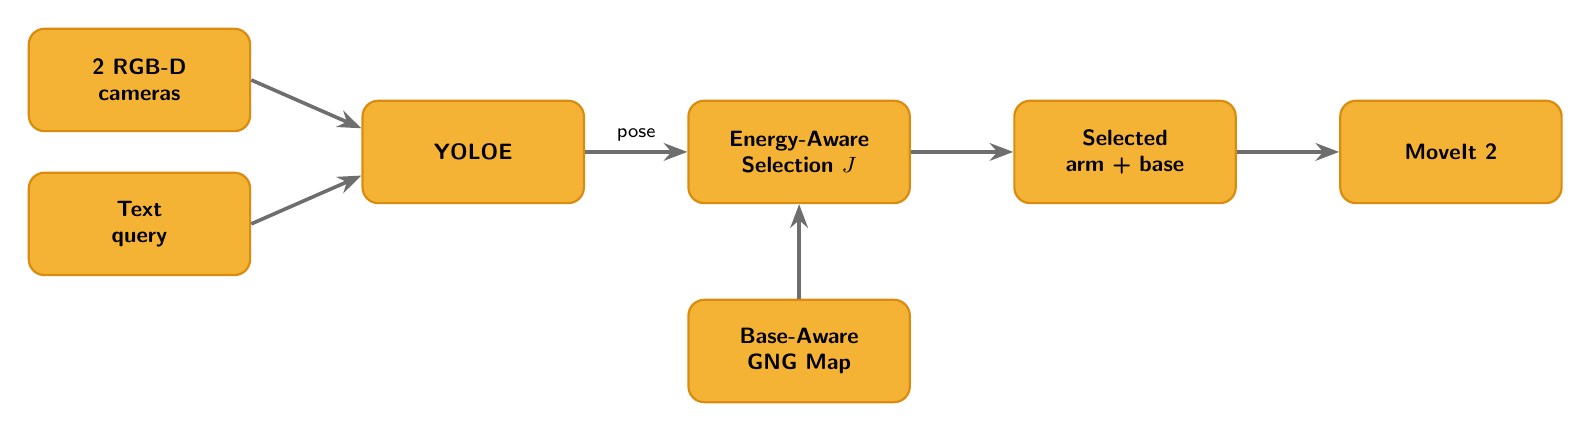
\begin{tikzpicture}[>=Stealth, thick, font=\footnotesize,
  box/.style={draw=pgoldd, fill=pgold, text=black, rounded corners=2mm,
              align=center, minimum height=13mm, text width=26mm, inner sep=3pt,
              font=\bfseries\footnotesize},
  arr/.style={-{Stealth[length=3mm]}, line width=1.3pt, draw=pgrey}]
  \node[box] (cam) {2 RGB-D\\cameras};
  \node[box, below=5mm of cam] (query) {Text\\query};
  \coordinate (m) at ($(cam.east)!0.5!(query.east)$);
  \node[box, right=14mm of m, anchor=west] (yolo) {YOLOE};
  \node[box, right=13mm of yolo] (sel) {Energy-Aware\\Selection $J$};
  \node[box, below=12mm of sel] (gng) {Base-Aware\\GNG Map};
  \node[box, right=13mm of sel] (arm) {Selected\\arm + base};
  \node[box, right=13mm of arm] (mv) {MoveIt~2};
  \draw[arr] (cam.east)   -- ([yshift=3mm]yolo.west);
  \draw[arr] (query.east) -- ([yshift=-3mm]yolo.west);
  \draw[arr] (yolo) -- node[above, font=\scriptsize] {pose} (sel);
  \draw[arr] (gng)  -- (sel);
  \draw[arr] (sel)  -- (arm);
  \draw[arr] (arm)  -- (mv);
\end{tikzpicture}}\par}
\vspace{1mm}

\begin{minipage}[t]{0.53\linewidth}
  \vspace{0pt}
  \IG{0.78}{Env_Isaac.png}
\end{minipage}\hfill
\begin{minipage}[t]{0.44\linewidth}
  \vspace{0pt}\RaggedRight
  All experiments run in \textbf{NVIDIA Isaac Sim}, a digital twin of our
  trailer living laboratory built from the \emph{same URDF} as the real robot.
  Two overhead RGB-D cameras are the only sensor: colour feeds detection, depth
  builds the collision octomap.
\end{minipage}

\psection{Perception Front End}

\begin{minipage}[t]{0.50\linewidth}
  \vspace{0pt}
  \IG{0.82}{Fig3YOLOE_RGBD.png}
\end{minipage}\hfill
\begin{minipage}[t]{0.47\linewidth}
  \vspace{0pt}\RaggedRight
  \textbf{YOLOE} segments each object from a free-form text prompt. Masked depth
  is back-projected and the \emph{median} world point taken as the centroid; the
  two cameras are fused by centroid proximity (0.10~m) and majority label
  voting. No fixed object database: ask by name.
\end{minipage}

\begin{keybox}
\lead{E4 --- YOLOE vs.\ Isaac ground truth} (8 objects, 483 frames):
\num{100\%} detection (3864/3864), mean localization error \num{0.023~m},
\num{0\%} false positives at conf $=0.25$.
\end{keybox}

\psection{Experiments and Results}

\lead{E1 --- the rail is worth $4\times$ the workspace.} Rail locked (6 arm DOF)
vs.\ rail sampled over its full travel, at matched sample \emph{density}:
reachable volume grows \num{1.920$\rightarrow$7.899~m$^3$} at 0.05~m voxels
(\num{$\approx4\times$}). \lead{E1b --- boundary seeding} cuts the node-hull
shortfall against the true FK reach surface from \num{0.221~m to 0.008~m}
(along the rail axis 0.501~m~$\rightarrow$~0.017~m).

\vspace{1mm}
{\centering\IG{0.80}{results.pdf}\par}
\figcap{(a) Reachable volume, rail locked vs.\ active. (b) Measured trajectory
energy per multi-arm policy ($\diamond$ = mean).}

\vspace{1mm}
\lead{E3 --- selection policies}, 60 target poses, plan-only, mean/median over
successful picks, under a rail friction model with assumed Coulomb/viscous terms
(a modelling assumption, not measured hardware data).

\vspace{1mm}
{\centering\fontsize{16}{20}\selectfont
\begin{tabular}{@{}l c c c@{}}
\toprule
\textbf{Mode} & \textbf{Success} & \textbf{Rail lin. (m)} & \textbf{Energy (J)}\\
\midrule
\textbf{energy (ours)} & \num{56/60 (93.3\%)} & \textbf{0.97}/1.01 & \num{\textbf{45.84}}/52.34\\
nearest                & 56/60 (93.3\%) & 1.19/1.41 & 48.28/54.79\\
random                 & 56/60 (93.3\%) & 1.17/1.28 & 47.31/51.72\\
fixed (best, arm\_4)   & 39/60 (65.0\%) & 1.14/1.21 & 49.79/55.78\\
fixed (worst, arm\_1)  & 38/60 (63.3\%) & 1.13/1.28 & 45.43/43.12\\
\bottomrule
\end{tabular}\par}
\figcap{Fixed-arm energies are computed over that arm's own smaller reachable
set, so they are not comparable at equal coverage.}

\begin{itemize}
  \item \lead{Coverage:} every multi-arm policy reaches \num{93.3\%} plan
        success vs.\ \num{63--65\%} for any single fixed arm.
  \item \lead{Energy:} ours has the \textbf{lowest mean measured energy} of the
        multi-arm policies (\num{45.84~J} vs.\ 48.28~J nearest, $-5.1\%$;
        47.31~J random, $-3.1\%$), winning \num{57--61\%} of same-target pairwise
        comparisons --- a real but \emph{partial} win: medians are closer and
        the distributions overlap.
  \item \lead{The intended trade appears:} ours spends \emph{more} arm travel
        to avoid costlier rail travel --- one logged pick took arm\_3 (0.64~m
        rail, 42.4~J) over the nearest arm\_4 (1.15~m rail, 72.5~J):
        \num{30.1~J} saved.
\end{itemize}

\psection{End-to-End Validation}

\begin{minipage}[t]{0.40\linewidth}
  \vspace{0pt}
  \IG{0.90}{fig5-pick_banana.png}
\end{minipage}\hfill
\begin{minipage}[t]{0.57\linewidth}
  \vspace{0pt}\RaggedRight
  \lead{E6:} perception $\rightarrow$ localization $\rightarrow$ energy-aware
  selection $\rightarrow$ IK $\rightarrow$ planning $\rightarrow$ real Isaac
  physics execution, on the 7 reachable objects $\times$ 5 trials:
  \num{35/35 (100\%)} picks, no failure in any category, mean time-to-pick
  \num{39.6~s}.

  \vspace{1.5mm}
  \lead{E5:} the map's nearest-node test classifies reachable vs.\ unreachable
  objects \num{100\% (8/8)} at \texttt{reach\_radius} $\geq0.12$~m, zero false
  positives.
\end{minipage}

\psection{Summary and Contributions}

\begin{keybox}
\begin{itemize}[leftmargin=6mm, topsep=0pt]
  \item An \textbf{energy-aware cost $J$} that picks the arm \emph{and} the full
        8-DOF configuration, rail travel included, instead of the nearest
        reachable pose.
  \item A \textbf{base-aware GNG capability map} treating the ceiling rail as a
        genuine DOF: every node carries its own rail placement and
        manipulability, accurate to \textbf{centimetres} at the workspace edge.
  \item An \textbf{Isaac Sim evaluation}: $\approx4\times$ workspace gain,
        93.3\% vs.\ 63--65\% plan success, lowest mean measured energy among
        multi-arm policies, 35/35 end-to-end picks.
\end{itemize}
\end{keybox}

\lead{Future work.} All results are in simulation. Next: validation on the
physical ceiling-rail platform, and how the sim-to-real gap shifts the
calibrated weights of $J$.

\end{minipage}

\vspace{3mm}
{\fontsize{13}{15.5}\selectfont\color{pgrey}
\textbf{References.}
[1]~Zacharias \textit{et al.}, IROS 2007.
[2]~Makhal \& Goins, IRC 2018 (Reuleaux).
[3]~Fritzke, NIPS 1995 (GNG).
[4]~Yoshikawa, IJRR 1985.
[5]~Sandakalum \textit{et al.}, Humanoids 2022.
[6]~Shao \textit{et al.}, arXiv:2403.19940 (MoMa-Pos).
[7]~Naik \textit{et al.}, IROS 2024 (BaSeNet).
[8]~Wang \textit{et al.}, ICCV 2025 (YOLOE).
[9]~Carpentier \textit{et al.}, SII 2019 (Pinocchio).
[10]~Coleman \textit{et al.}, JOSER 2014 (MoveIt).
\par}

\end{document}
